% Source: StudentGovernmentRepo/Common_Sense_Carolina_Lobbying_org/figures/timeline.tex
\documentclass[border=25pt]{standalone}
\usepackage{tikz}
\usepackage{xcolor}
\usetikzlibrary{positioning, arrows.meta, calc, fit, backgrounds, decorations.markings}
\definecolor{garnet}{HTML}{73000A}
\definecolor{sandstorm}{HTML}{FFF2E3}
\definecolor{rose}{HTML}{CC2E40}
\definecolor{atlantic}{HTML}{466A9F}
\definecolor{congaree}{HTML}{1F414D}
\definecolor{horseshoe}{HTML}{65780B}
\definecolor{honeycomb}{HTML}{A49137}
\definecolor{warmgrey}{HTML}{676156}
\definecolor{tenblack}{HTML}{ECECEC}

\begin{document}
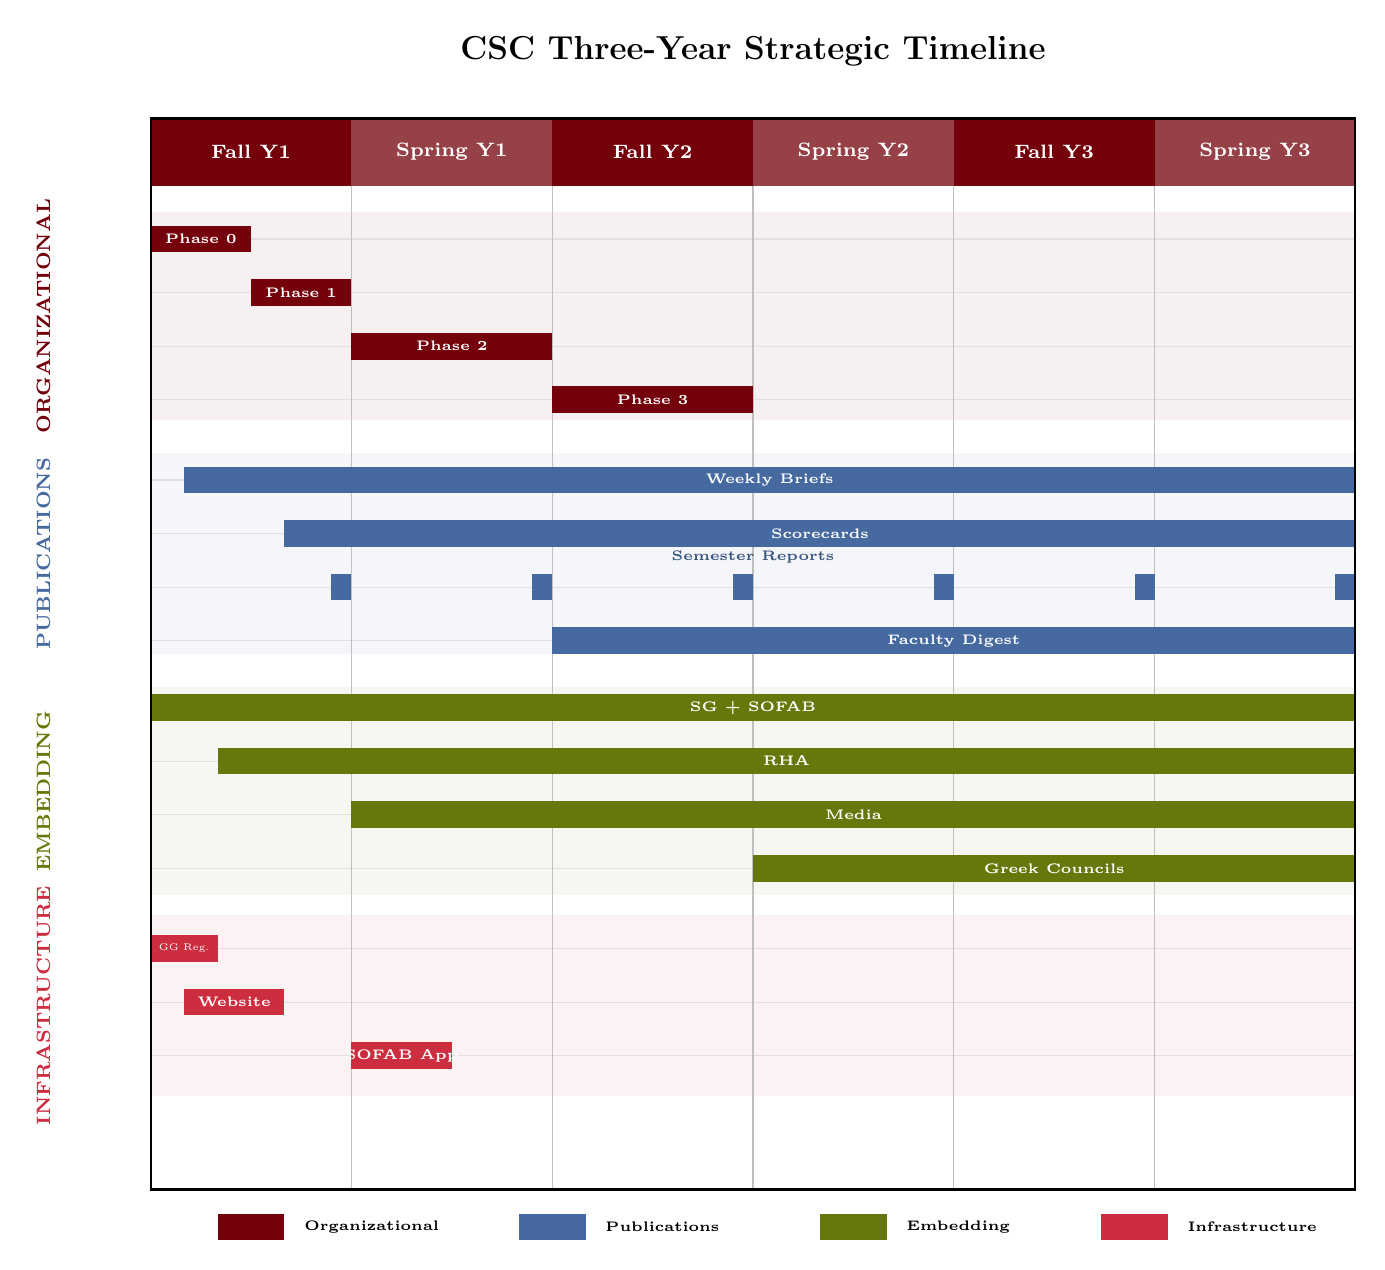
\begin{tikzpicture}[x=0.85cm, y=0.85cm]

%--- Section background bands (drawn first, behind everything)
\fill[garnet!6]    (0, 11.5) rectangle (18, 14.6);
\fill[atlantic!6]  (0,  8.0) rectangle (18, 11.0);
\fill[horseshoe!6] (0,  4.4) rectangle (18,  7.5);
\fill[rose!6]      (0,  1.4) rectangle (18,  4.1);

%--- Light horizontal grid lines at bar vertical midpoints
\foreach \y in {14.2, 13.4, 12.6, 11.8, 10.6, 9.8, 9.0, 8.2, 7.2, 6.4, 5.6, 4.8, 3.6, 2.8, 2.0} {
  \draw[black!12, thin] (0, \y) -- (18, \y);
}

%--- Vertical grid lines at semester boundaries
\foreach \x in {0,3,6,9,12,15,18} {
  \draw[black!25, thin] (\x, 0) -- (\x, 15);
}

%--- HEADER ROW
\fill[garnet]     (0,15) rectangle  (3,16);
\fill[garnet!75]  (3,15) rectangle  (6,16);
\fill[garnet]     (6,15) rectangle  (9,16);
\fill[garnet!75]  (9,15) rectangle (12,16);
\fill[garnet]    (12,15) rectangle (15,16);
\fill[garnet!75] (15,15) rectangle (18,16);

\node[white, font=\scriptsize\bfseries] at  (1.5,15.5) {Fall Y1};
\node[white, font=\scriptsize\bfseries] at  (4.5,15.5) {Spring Y1};
\node[white, font=\scriptsize\bfseries] at  (7.5,15.5) {Fall Y2};
\node[white, font=\scriptsize\bfseries] at (10.5,15.5) {Spring Y2};
\node[white, font=\scriptsize\bfseries] at (13.5,15.5) {Fall Y3};
\node[white, font=\scriptsize\bfseries] at (16.5,15.5) {Spring Y3};

%--- SECTION LABELS (rotated, left of chart)
\node[garnet,   font=\scriptsize\bfseries, rotate=90] at (-1.6, 13.05) {ORGANIZATIONAL};
\node[atlantic, font=\scriptsize\bfseries, rotate=90] at (-1.6,  9.5)  {PUBLICATIONS};
\node[horseshoe,font=\scriptsize\bfseries, rotate=90] at (-1.6,  5.95) {EMBEDDING};
\node[rose,     font=\scriptsize\bfseries, rotate=90] at (-1.6,  2.75) {INFRASTRUCTURE};

%=== SECTION 1: ORGANIZATIONAL (garnet bars) ===
% Phase 0: x=0-1.5, y=14-14.4
\fill[garnet] (0,14) rectangle (1.5,14.4);
\node[white, font=\tiny\bfseries] at (0.75,14.2) {Phase 0};

% Phase 1: x=1.5-3, y=13.2-13.6
\fill[garnet] (1.5,13.2) rectangle (3,13.6);
\node[white, font=\tiny\bfseries] at (2.25,13.4) {Phase 1};

% Phase 2: x=3-6, y=12.4-12.8
\fill[garnet] (3,12.4) rectangle (6,12.8);
\node[white, font=\tiny\bfseries] at (4.5,12.6) {Phase 2};

% Phase 3: x=6-9, y=11.6-12.0
\fill[garnet] (6,11.6) rectangle (9,12.0);
\node[white, font=\tiny\bfseries] at (7.5,11.8) {Phase 3};

%=== SECTION 2: PUBLICATIONS (atlantic bars) ===
% Weekly Briefs: continuous from x=0.5-18
\fill[atlantic] (0.5,10.4) rectangle (18,10.8);
\node[white, font=\tiny\bfseries] at (9.25,10.6) {Weekly Briefs};

% Scorecards: x=2-18
\fill[atlantic] (2,9.6) rectangle (18,10.0);
\node[white, font=\tiny\bfseries] at (10,9.8) {Scorecards};

% Semester Reports — small end-of-semester blocks
\foreach \xs/\xe in {2.7/3, 5.7/6, 8.7/9, 11.7/12, 14.7/15, 17.7/18} {
  \fill[atlantic] (\xs,8.8) rectangle (\xe,9.2);
}
% Label positioned between two blocks for readability
\node[atlantic!80!black, font=\tiny\bfseries] at (9,9.45) {Semester Reports};

% Faculty Digest: x=6-18
\fill[atlantic] (6,8.0) rectangle (18,8.4);
\node[white, font=\tiny\bfseries] at (12,8.2) {Faculty Digest};

%=== SECTION 3: EMBEDDING (horseshoe bars) ===
% SG + SOFAB: full span
\fill[horseshoe] (0,7.0) rectangle (18,7.4);
\node[white, font=\tiny\bfseries] at (9,7.2) {SG + SOFAB};

% RHA: x=1-18
\fill[horseshoe] (1,6.2) rectangle (18,6.6);
\node[white, font=\tiny\bfseries] at (9.5,6.4) {RHA};

% Media: x=3-18
\fill[horseshoe] (3,5.4) rectangle (18,5.8);
\node[white, font=\tiny\bfseries] at (10.5,5.6) {Media};

% Greek Councils: x=9-18
\fill[horseshoe] (9,4.6) rectangle (18,5.0);
\node[white, font=\tiny\bfseries] at (13.5,4.8) {Greek Councils};

%=== SECTION 4: INFRASTRUCTURE (rose bars) ===
% Garnet Gate Reg.: x=0-1
\fill[rose] (0,3.4) rectangle (1,3.8);
\node[white, font=\tiny] at (0.5,3.6) {\scalebox{0.7}{GG Reg.}};

% Website Launch: x=0.5-2
\fill[rose] (0.5,2.6) rectangle (2,3.0);
\node[white, font=\tiny\bfseries] at (1.25,2.8) {Website};

% SOFAB App: x=3-4.5
\fill[rose] (3,1.8) rectangle (4.5,2.2);
\node[white, font=\tiny\bfseries] at (3.75,2.0) {SOFAB App};

%--- Outer border
\draw[black, thick] (0,0) rectangle (18,16);

%=== LEGEND ===
\def\ly{-0.75}
\def\lh{0.38}

\fill[garnet]    (1.0,\ly) rectangle (2.0,\ly+\lh);
\node[font=\tiny\bfseries, anchor=west] at (2.15,\ly+\lh/2) {Organizational};

\fill[atlantic]  (5.5,\ly) rectangle (6.5,\ly+\lh);
\node[font=\tiny\bfseries, anchor=west] at (6.65,\ly+\lh/2) {Publications};

\fill[horseshoe] (10.0,\ly) rectangle (11.0,\ly+\lh);
\node[font=\tiny\bfseries, anchor=west] at (11.15,\ly+\lh/2) {Embedding};

\fill[rose]      (14.2,\ly) rectangle (15.2,\ly+\lh);
\node[font=\tiny\bfseries, anchor=west] at (15.35,\ly+\lh/2) {Infrastructure};

%=== TITLE ===
\node[font=\large\bfseries] at (9,17) {CSC Three-Year Strategic Timeline};

\end{tikzpicture}
\end{document}
